\section{Hamiltonian 学习与共振分析}
\label{sec:learning-kam}

\subsection{具有复可训练表示的实能量}
Hamiltonian 学习通过对标量能量求导获得保守向量场\citep{Greydanus2019,Chen2022}。本节的目标为具有理想均匀轴向磁偏置的变质量 Kirchhoff 模型，记为 $H_{\mathrm{ideal}}$；该模型有 12 个配置自由度、24 维相空间和 20 个几何积分单元。完整线圈系统采用另一磁势。这些保守标签不含流体、接触和阻尼力。因此，学习实验检验的是所声明机械能量的近似，而部署还需要物理端口接口。

采用无量纲正则状态 $z=(Q,P)$、能量 $h=H/E_0$ 和时间 $\tau=\omega_0t$。在物理正则缩放之后定义
\begin{equation}
 \begin{aligned}
 \xi&=(Q+iP)/\sqrt2,\\
 \chi&=(Q-iP)/\sqrt2.
 \end{aligned}
 \label{eq:learn-complex-coordinate}
\end{equation}
实切片上 $\chi=\bar\xi$，全纯延拓时二者独立。逆变换给出
\begin{equation}
 \begin{aligned}
 \partial_\chi&=(\partial_Q+i\partial_P)/\sqrt2,\\
 \{\xi_j,\chi_k\}&=-i\delta_{jk},\\
 \xi'&=-ih_\chi+iR/\sqrt2,
 \end{aligned}
 \label{eq:learn-complex-field}
\end{equation}
其中 $R$ 作用于动量方程。训练损失与预测器必须采用同一导数约定。复参数不会使物理能量成为复值函数，仅设置能量虚部输出也不能实现物理 Rayleigh 阻尼。

训练采用 $x=Dz$，其中 $D=\operatorname{diag}(\sqrt\nu,\sqrt\nu)/a$、$\nu=\omega/\omega_0$、$a=0.08$。这一附加缩放不是正则变换：$\nabla_zh=D\nabla_xh$，且 $x'=DJD\nabla_xh$。所有模型均增加残差 $r_\theta$，其基底为同一二次先验 $h_2=a^2\|x\|^2/2$。

有限解析模型包含动量次数为零或二的全部三次、四次机械残差：$Q^3$、$Q^4$、$QP^2$ 和 $Q^2P^2$，分别贡献 364、1365、936 和 6084 个系数。这 8749 个实参数描述所声明的机械函数类，而非 24 变量的全部四次多项式。完整复网络具有两个宽度为 48 的复隐藏层和一个复读出，共 3552 个复参数，即 7104 个实参数。网络同时使用复输入及其共轭、分离激活 $\sigma(u)=\tanh(\operatorname{Re}u)+i\tanh(\operatorname{Im}u)$、三次门控及 $P\mapsto-P$ 平均。所有权重的实部和虚部均参与训练。门控保留二次先验，平均保留动量偶性；二者均不保证关于动量的凸性。

机械复网络使用 13440 个实参数，预测下三角矩阵 $L(Q)$ 及势能残差；矩阵具有正指数对角元并满足 $L(0)=I$。其能量为
\begin{equation}
 \begin{aligned}
 h_\theta&=\tfrac12a^2x_P^TLL^Tx_P\\
 &\quad+\tfrac12a^2\|x_Q\|^2+V_\theta(x_Q),\\
 (h_\theta)_{PP}&=D_\nu LL^TD_\nu,
 \end{aligned}
 \label{eq:learn-spd}
\end{equation}
其中 $D_\nu=\operatorname{diag}\sqrt\nu$。对有限实输出，有 $v^T(h_\theta)_{PP}v=\|L^TD_\nu v\|^2>0$，对任意 $v\ne0$ 均成立。因此在精确算术下，固定 $Q$ 的动量到速度映射是线性双射。这证明了结构性质，但未给出统一条件数或物理质量误差界。

分离激活是实解析的，但并非单复变量全纯函数。合法延拓将共轭输入替换为独立变量，并使用
\begin{equation}
 \begin{aligned}
 \sigma^{\mathbb C}(u,v)&=\tanh((u+v)/2)\\
 &\quad+i\tanh((u-v)/(2i)),
 \end{aligned}
 \label{eq:learn-analytic-extension}
\end{equation}
同时冻结训练系数及其共轭。这样在避开所有层极点的域内得到局部全纯延拓。所报告的训练并未认证统一极点裕量或复域近似范数。

\subsection{冻结训练与机械诊断}
实验以数据种子 51001 在 $[-1,1]^{24}$ 内均匀抽取 1024 个训练状态和 256 个验证状态。每种架构分别采用种子 51001--51003，进行 1200 次 Adam 更新，批量大小为 128。多项式与网络的学习率分别为 $10^{-3}$ 和 $3\times10^{-3}$，梯度裁剪阈值为 10。令 $r_*=h_{\mathrm{ideal}}-h_2$，实际目标函数为
\begin{equation}
 \begin{aligned}
 \mathcal L&=\operatorname{mean}\left[\left(\frac{D(\nabla_xr_\theta-\nabla_xr_*)}{s_g}\right)^2\right]\\
 &\quad+0.15\operatorname{mean}\left[\left(\frac{r_\theta-r_*}{s_h}\right)^2\right],
 \end{aligned}
 \label{eq:learn-objective}
\end{equation}
其中 $s_h=0.00954395736$ 为训练残差能量标准差，$s_g=0.4661470702$ 为其正则梯度均方根。验证集每 50 次更新选择检查点，同时检查第一次更新。九组权重全部冻结之后，才以种子 510990 生成 $[-1,1]^{24}$ 内的 512 个独立测试标签和 $[-1.5,1.5]^{24}$ 内的 256 个扩展域标签。计算采用 float64/complex128、单 CPU 线程和 PyTorch 2.5.1；记录的本次运行耗时约 410.8\,s。

表~\ref{tab:learn-errors} 和图~\ref{fig:learning} 报告各样本集上的正则场相对 $L^2$ 误差 $\|J\nabla(h_\theta-h_*)\|_2/\|J\nabla h_*\|_2$。在本预算下，无约束复网络精度最高，而仅 SPD 模型保证正动量曲率。二次先验的测试误差为 63.094\%，较小的历史 48 特征读出为 62.964\%。参数数量、函数类、学习率与每次更新成本不同，因此这些比较不能单独识别复参数化相对实参数化的优势。尤其是，有限预算 Adam 并不证明已达到多项式类的最小二乘最优解。

\begin{table*}[t]
 \centering
 \caption{冻结学习结果：三个种子的范围。最后一列为每个种子在八个预先指定测试状态上的非正动量 Hessian 数量。扩展域使用放大 1.5 倍的坐标盒。}
 \label{tab:learn-errors}
 \small\setlength{\tabcolsep}{3.5pt}
 \begin{tabular}{lrrrr}
 \toprule
 模型 & 实参数数 & 测试场误差 (\%) & 扩展域误差 (\%) & 非正 $h_{PP}$ \\
 \midrule
 机械多项式 & 8749 & 35.249--35.282 & 59.743--60.273 & 4/4/4 \\
 完整复隐藏层 & 7104 & 3.241--3.700 & 8.410--9.063 & 2/2/4 \\
 SPD 机械复网络 & 13440 & 11.415--11.553 & 20.651--21.917 & 0/0/0 \\
 \bottomrule
 \end{tabular}
\end{table*}

对每个种子的八个测试状态与八个扩展域状态，分别检查 Hessian、能量二阶差分及 Legendre 方程 $\partial_Ph_\theta(Q,\widehat P)=\partial_Ph_*(Q,P)$。以真实 $P$ 初始化使其成为有利的局部检验。方程残差很小仍可伴随较大的恢复动量误差。部分求解器进展标志为假，但残差已接近舍入量级；无约束复模型还存在实质非零的反解残差。其测试样本中最大的 Hessian 条件数达到 $1.67\times10^5$。SPD 模型扩展域样本的条件数最大约为 1811；正定性不等于惯量准确。多项式、复网络和 SPD 模型的测试样本最大 Hessian 相对误差依次为 47.49\%、5.82\% 和 17.05\%，最大相对恢复动量误差依次为 27.30、0.6267 和 0.5044。独立重新生成的标签和方向二阶差分确认了保存的负曲率符号。

部署所需的学习场修正为 $(-\delta g_P,+\delta g_Q)$，其中 $\delta g=\nabla h_\theta-\nabla h_*$。线圈电流仅直接改变动量方程。因此，独立的受限分配测试 $\delta g_Q$ 的可达部分，同时保留配置速度误差和线圈像空间外的力分量。三个模型、三个种子和八个状态的全部 72 项修正分配均完成；在相对阈值 $10^{-8}$ 下，端口有效秩为五，部分电流达到 2\,A 边界。多项式、复网络和 SPD 模型修正后与修正前的总场误差比依次为 0.8845--0.9898、0.8959--0.9960 和 0.8482--0.9965。该实验是在声明的 0.25\,s 电流变化窗口下进行的静态分配诊断，没有积分学习闭环。


\begin{figure*}[t]
\centering
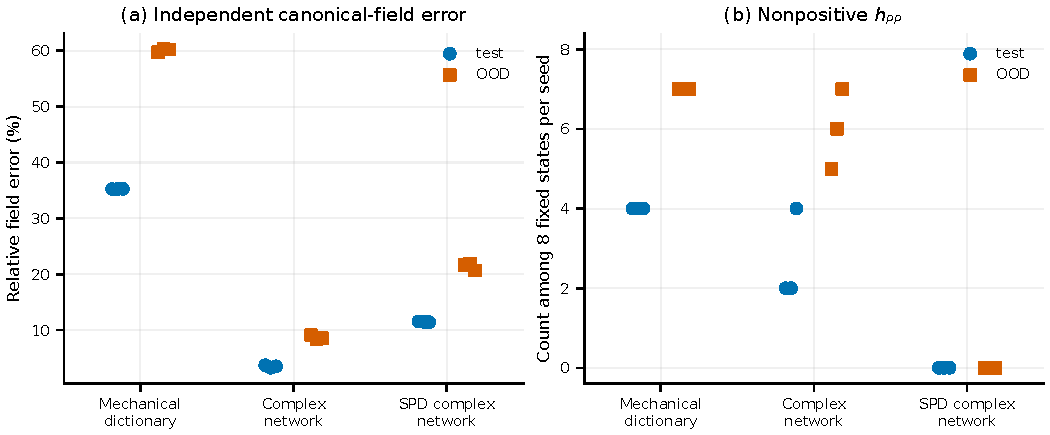
\includegraphics[width=\textwidth]{../figures/learning.pdf}
\caption{冻结 Hamiltonian 学习比较。每个点对应三个训练种子之一；左图为独立测试域及域外的正则向量场误差，右图为每个种子在各数据分区的八个预定状态中非正动量 Hessian 的数量。这些有限样本不构成统一域界。所有模型均针对理想偏置 Hamiltonian 训练，而非完整线圈磁势。}
\label{fig:learning}
\end{figure*}

\subsection{从经验误差到持久性假设}
两条不同的误差论证保留学习与动力学之间的联系。对有限基，写作 $h_\theta=h_0+\sum c_{\theta j}\psi_j$、$h_*=h_0+\sum c_{*j}\psi_j+R$。将样本导数特征堆叠成 $A$，去除常数规范，并对所有残差采用同一观测归一化 $N_o$。若 $G=A^TA/N_o\succeq\lambda I$，则
\begin{equation}
 \begin{aligned}
 \|h_\theta-h_*\|_{\mathcal X}
 &\le B_{\mathcal X}\frac{r+e}{\sqrt\lambda}+\|R\|_{\mathcal X},\\
 B_{\mathcal X}&=\Big(\sum_j\|\psi_j\|_{\mathcal X}^2\Big)^{1/2}.
 \end{aligned}
 \label{eq:learn-gram-bound}
\end{equation}
其中 $r$ 是拟合观测残差，$e$ 包含观测误差与 $R$ 的样本导数。证明只使用最小奇异值与 Cauchy--Schwarz 不等式，不要求样本独立或拟合达到最优。范数可以是实域 $C^\ell$ 范数，也可以是指定复域上的解析上确界范数。积分观测需计入端点与求积误差，导出系数需计入舍入界。旧两模态完整余弦模型保留全部 35 个四次方向，由一个余弦系数和 34 个正交多项式方向实现。其 Gram 下界不能移用于新的 8749 特征字典。

另一条条件性论证\citep{Chen2022}结合参数覆盖、Hoeffding 集中、Poincar\'e 不等式和插值。设 $\mathcal D=\mathbb T^n\times B$、$d=2n$、$p>d$、$\ell\ge1$，且整数 $s>\ell+d/p$。要求独立样本的密度至少为 $m_0$、实化参数位于有界立方体、梯度残差和参数 Lipschitz 常数具有统一界，且固定规范后存在统一 $W^{s,p}$ 界 $M_s$。则以至少 $1-\delta$ 的概率，对整个函数类同时成立
\begin{equation}
 \begin{aligned}
 \|e_\theta\|_{C^\ell}&\le E_\theta,\\
 E_\theta&=C_{\mathrm{GN}}(G_\theta+M_s^\alpha G_\theta^{1-\alpha}),\\
 \alpha&=\frac{\ell-1+d/p}{s-1},
 \end{aligned}
 \label{eq:learn-statistical-bound}
\end{equation}
其中 $G_\theta=C_Pm_0^{-1/p}(\widehat R_\theta+\Gamma)^{1/p}$，$\Gamma$ 是补充材料推导的显式覆盖惩罚。这是统一统计蕴含，而非 Adam 收敛定理。对当前网络，两条论证所需的常数均未全部认证。有限样本梯度误差本身不能补足这些常数：仅在单个标量变量 $w$ 中，多项式 $c\prod_j(w-w_j)^2$ 就能在样本点保持函数值和一阶导数为零，而复域范数可随 $c$ 任意增大。

\begin{figure*}[t]
\centering
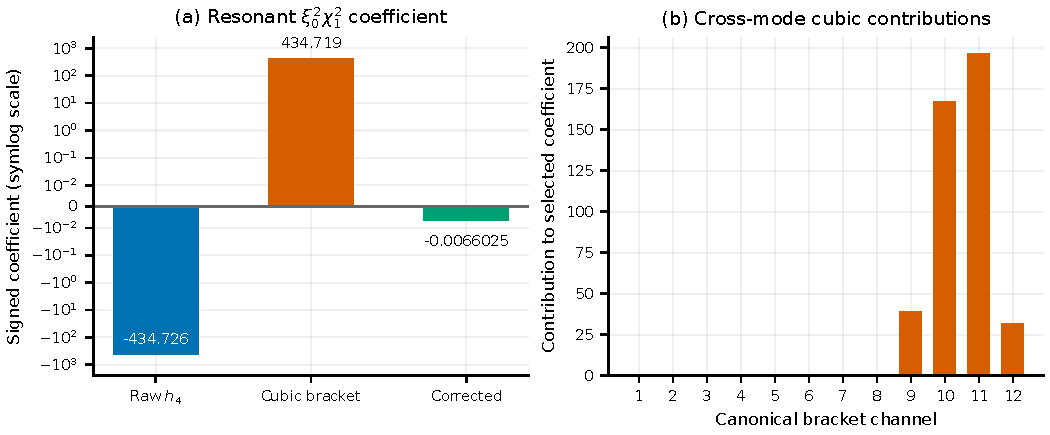
\includegraphics[width=\textwidth]{../figures/resonance.pdf}
\caption{第一频率对四次共振诊断。左图以对称对数尺度显示原四次系数、保留全部12个括号通道的三次消去修正及其较小残差；右图为四个外部扭转括号通道对三次消去修正的贡献，通道从一开始编号。计算保留了全部12个正则通道。原第一频率对子空间并不不变，因此这一受限系数不能证明完整系统的 KAM 非退化性。}
\label{fig:resonance}
\end{figure*}

\subsection{共振的三维机械模型}
实际理想偏置模型的线性化具有四对 $1{:}1$ 弯曲频率，其频率比分别为 $1$、$6.21276315$、$17.89814255$ 和 $80.07400435$。在阈值 $10^{-10}$ 下，全部 2600 个三次单项式中无共振，最小除数为一；17550 个四次单项式中有 206 个位于同调核，包括 78 个作用量项和 128 个非作用量项。成对简并来自圆杆的轴向对称性；数值阈值只是有限阶诊断。

对 $h=h_2+h_3+h_4+\cdots$、$h_2=\sum_j\nu_j\xi_j\chi_j$，同调方程及其三次解为
\begin{equation}
 \begin{aligned}
 \{h_2,\xi^\alpha\chi^\beta\}
 &=i\nu\cdot(\alpha-\beta)\xi^\alpha\chi^\beta,\\
 (W_3)_{\alpha\beta}&=\frac{i(h_3)_{\alpha\beta}}{\nu\cdot(\alpha-\beta)}.
 \end{aligned}
 \label{eq:learn-homological}
\end{equation}
于是 $\{h_2,W_3\}=-h_3$，Lie 展开给出共振四次项
\begin{equation}
 Z_4=\Pi_{\mathrm{res}}\left(h_4+\tfrac12\{h_3,W_3\}\right).
 \label{eq:learn-resonant-quartic}
\end{equation}
限制到第一对弯曲模态时，仍保留全部 12 个正则括号通道。对完整梯度沿选定四个实坐标求两次导数，即可获得在一次求导后仍能对该限制贡献的所有三次单项式；含两个外部变量的项不能贡献。四个外部扭转通道为 $\xi_0^2\chi_1^2$ 系数提供非零修正：
\begin{equation}
 \begin{aligned}
 &-434.7256304212535+434.719027922014\\
 &\qquad\simeq-0.006602499239534154.
 \end{aligned}
 \label{eq:learn-cancellation}
\end{equation}
该抵消超过四个数量级（图~\ref{fig:resonance}）。采用的计算使用反向自动微分，四阶置换缺陷为 $2.27\times10^{-13}$，并通过独立标量求导检查。其原始系数与半径外推之差为 $7.26\times10^{-7}$。先前混合模式导数张量未通过置换对称性检验（缺陷为 1738.9），因此未采用；失败文件仍保留。这些检查验证有限阶数值一致性，没有界定解析尾项或抵消过程中的舍入误差。

计算所得限制满足下式，系数缺陷为 $1.23\times10^{-13}$：
\begin{equation}
 \begin{aligned}
 Z_{4,\mathrm{pair}}&=A(I_0+I_1)^2+BL^2,\\
 L&=Q_0P_1-Q_1P_0,
 \end{aligned}
 \label{eq:learn-pair-form}
\end{equation}
其中 $I_j=\xi_j\chi_j$、$A=0.0004112209869572539$、$B=0.006602499239534154$。酉变换 $\xi_\pm=(\xi_0\mp i\xi_1)/\sqrt2$ 的实化是辛变换，其作用量为 $I_\pm=(N\pm L)/2$，$N=I_0+I_1$。因此形式扭转的特征值为 $4A\simeq0.00164488$、$4B\simeq0.0264100$，行列式为 $16AB\simeq4.34414\times10^{-5}$。32 个状态上的独立检查给出最大作用量恒等式误差 $8.67\times10^{-19}$。然而，原第一对坐标子空间中三个状态的外模态场范数为 0.01643、0.06573 和 0.26300。该子空间不由完整非线性动力学保持。因此，该计算建立的是受限四次候选，而非两自由度物理子系统或全维扭转。一个轴向 $SO(2)$ 动量也不能提供四个独立对称约化；正则约化要求自由作用和正则动量水平，而直杆平衡点不满足这些条件。




\subsection{连续与离散 KAM 的范围}
连续持久性要求：指定正则域上的保守 Hamiltonian、频率映射具有有界逆的可积主部、足够正则性、边界裕量、Diophantine 界 $|k\cdot\omega|\ge\gamma|k|^{-\tau}$（对所有 $k\ne0$ 成立），以及所选定理的小量阈值\citep{Poschel2001}。若同一图上 $h_*=h_0+P_*$、$h_\theta=h_0+P_\theta$，则固定规范后学习扰动的认证界 $\beta_\theta$ 与误差界 $E_\theta$，须在相应定理假设下共同满足 $\beta_\theta+E_\theta<c_K\gamma^2$。分别应用定理可得两套环面族，并不意味着嵌入相同。物理扰动和正规形余项仍属于该预算。

离散持久性还要求在保留域上的解析 exact-symplectic 映射及其逆、周期生成函数、离散扭转和频率裕量，以及
\begin{equation}
 |e^{i\Delta k\cdot\omega}-1|\ge\Delta\gamma_D|k|^{-\tau_D}\quad(k\ne0).
 \label{eq:learn-discrete-divisor}
\end{equation}
生成函数扰动须除以 $\Delta$ 后再与 Hamiltonian 界比较\citep{Shang1999}。小步长本身不能排除 $\Delta k\cdot\omega=2\pi m$。精确隐式方程的辛性也不意味着有限容差求解器就是 exact-symplectic 映射。继承的有限幅值证书针对某个冻结的两模态 Hamiltonian，使用其自身 Fourier 候选和验证域计算；它不为当前任一种三维磁势提供证书。这里尚未认证完整共振耦合、扭转逆、域与余项界，以及连续和离散小除数常数。
